\section{Sistema de respuesta a preguntas (Q\&A)}

\subsection{Descripción del problema}

Los sistemas de respuesta a preguntas (o Q\&A por sus siglas en ingles) integran tareas de recuperación de la información (IR) y procesamiento del lenguaje natural (NLP) para poder responder de forma automática a preguntas de un usuario. La primera tarea busca encontrar información relevante, que pueda contener la respuesta para el usuario (i.e. un documento), por medio de una herramienta de búsqueda. Ya con esta información (también llamada \textit{contexto}) un sistema de \textit{based QA} realiza la tarea de comprensión de lectura, con la cual se busca extraer la respuesta exacta a la pregunta del usuario \cite{}.
Esta segunda tarea tienen como único objetivo encontrar un pasaje (\textit{p}) que responda a la pregunta (\textit{q}) dentro del (o los) documentos relevantes recuperados para la pregunta. \\

A pesar de los recientes y acelerados desarrollos en el campo del procesamiento de lenguaje natural, los sistemas de respuesta a preguntas existen desde la década de los 60s. En esta época los sistemas se dedicaban a responder únicamente preguntas de un dominio muy especifico como baseball \cite{} o análisis geológico \cite{}. No obstante, con la gran cantidad de información disponible y el poder computacional de hoy en día, se puede fácilmente acceder a grandes colecciones de datos que permiten construir sistemas de respuesta a preguntas de dominio abierto. Asimismo, se tienen modelos de NLP profundos que permiten resolver de mejor forma la extracción de la respuesta dado el contexto.

\subsection{Revisión del estado del arte}

Para resolver el problema de recuperación de la información (IR) existen enfoques que datan desde la década de los 70s. Vale la pena aclarar que para esta tarea en especifico se requiere un \textit{set} ordenado de documentos (\textit{ranked}) y no solamente una colección de documentos relevantes y otros no. De esta manera se obtienen \textit{scores} de similaridad entre documento y \textit{query} para poder ordenar los resultados de la búsqueda. Con esto en mente, el enfoque más sencillo es el de utilizar la similaridad coseno de modelo de Bag-of-Words (BOW) que representa tanto al \textit{query} como al documento \cite{}. Mejoras a esta metodología incluyen pesar los documentos por frecuencia (\textit{tf-idf term weighting}) y puntuación de documentos (\textit{document scoring}) \cite{}. Hoy en día existen sistemas de IR bien establecidos como \textit{Lucene} \cite{lucene} y arquitecturas basadas en \textit{deep learning} para la recuperación de la información \cite{DL_IR}. \\

Por otro lado, los sistemas de comprensión de lectura (o \textit{based QA}) del estado del arte utilizan como base modelos contextuales profundos pre-entrenados como ELMo y BERT \cite{BertQA}. Esto se debe al gran desempeño que han demostrado estos modelos en un amplio espectro de tareas de NLP. Ahora bien, con el objetivo de adaptar estos modelos contextuales a la tarea especifica, se utiliza el \textit{dataset} de pregunta a respuestas estándar de la universidad de Standford SQuAD \cite{squad}. De esta manera, se realiza un \textit{fine-tuning} del modelo de BERT para así, a partir de su representación de la entrada (contexto y pregunta), el modelo recupere el pasaje con la respuesta \cite{BERT_on_SQUAD}.

\subsection{Metodología de solución}

La metodología general para la solución del problema de respuesta a preguntas se presenta en la figura \ref{fig:qa_diag}. Para esto se utilizó un subset de datos recopilados para Covid. Dada la naturaleza de la tarea en cuestión, los documentos recopilados de las redes sociales Twitter y Reddit fueron descartados, pues estas no proveen un contexto adecuado para la respuesta de preguntas y muchas veces dan información que es engañosa o falsa. Adicionalmente, se recopilo información de autoridades en la materia que brinden información adecuada y verídica para un tema tan sensible como lo es el Covid. En total se recuperaron entre 100 y 200 documentos de las páginas oficiales de la WHO y la CDC. \\

A estos documentos se les realizó un pre-procesamiento estándar que incluye:
\begin{itemize}
    \item \textbf{lower case:} Las letras de todos los términos se transformaron a minúsculas.
    
    \item \textbf{tokenización:} Se tokenizaron las palabras con el tokenizador \texttt{RegexpTokenizer} de \texttt{nltk}, el cual elimina todo signo de puntuación.
        
    \item \textbf{simple lematization:} Se redujo cada uno de los términos a su raíz con el lematizador \texttt{WordNetLematizer} de \texttt{nltk}.
\end{itemize}

\begin{figure}[H]
    \centering
    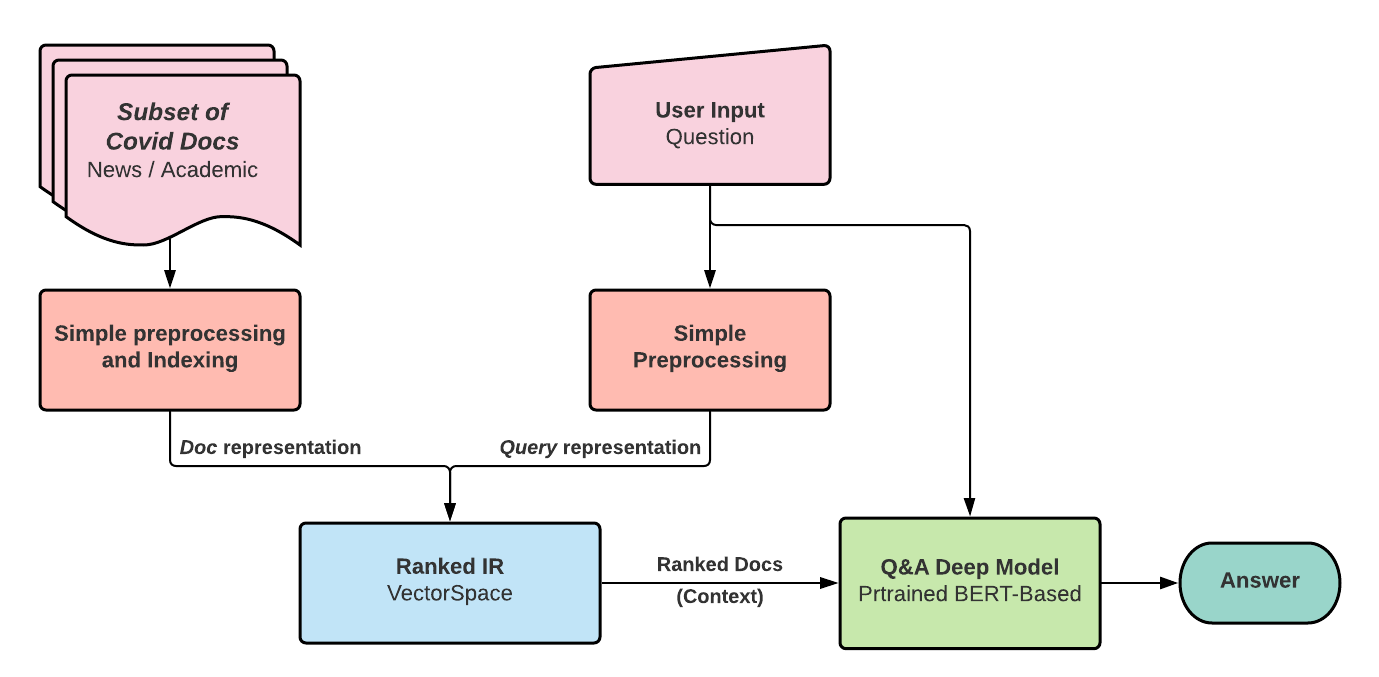
\includegraphics[width=\textwidth]{doc_final/images/QA_System_diag.png}
    \caption{Flujo de información Sistema de respuesta a preguntas}
    \label{fig:qa_diag}
\end{figure}

\subsubsection{Information Retrieval}

Una vez se tienen los documentos preprocesados, se procede a construir, entonces, el sistema de recuperación de la información (IR) con la librería de \texttt{Gensim}. Esta implementación realiza una vectorización de documentos de forma sencilla con un modelo de Tf-idf (\texttt{TfidfModel()}) con el corpus de documentos. Se crea una matriz de similaridad ((\texttt{MatrixSimilarity()}) con el modelo de Tf-idf del corpus de documentos. Con esta matriz y el modelo de Tfidf se transforman cada una de las \textit{queries} y se realiza la recuperación de la información a partir de su similaridad de coseno (\textit{cosine similarity score)}, ordenando los resultados de mayor a menor similaridad. De igual forma, se tienen en cuenta únicamente los documentos con un puntaje (\textit{score}) mayor a 0. Por último, estos documentos se pasan como contexto al modelo contextual profundo pre-entrenado. \\

\subsubsection{Q\&A Deep Model}

Ya con el contexto recuperado, se utiliza un modelo contextual pre-entrenado para la tarea de respuesta a preguntas (\textit{question-answering}), con el fin de extraer la respuesta como un pasaje del contexto. Para esto se consideraron los siguientes modelos:

\begin{itemize}
    \item Inglés: RoBerta-base SQuAD2.0 for QA on COVID-19
    
    \item Español: BETO (Spanish BERT) + Spanish SQuAD2.0
    
    \item Francés: CamemBERT model fine-tuned on FQuAD
\end{itemize}

Note que el modelo utilizado para inglés no solo se entrenó (\textit{fine-tuned}) con el \textit{dataset} para pregunta a respuestas SQuAD2.0 sino que también fue entrenado con un \textit{dataset} especifico para Q\&A en el dominio de COVID-19 \cite{}

% --------------------------------------------------------------------
%                                RESULTS
% --------------------------------------------------------------------
\subsection{Resultados}


\subsection{Conclusiones}

\newpage